% !TeX root = ../main.tex
\section{Структурная схема устройства}

Структурная схема тракта цифрового приема и согласованной фильтрации представлена на рисунке \ref{fig:block_diag}.

\begin{figure}[H]
    \centering
    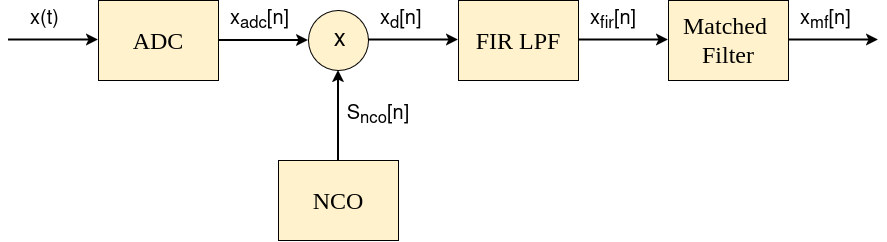
\includegraphics[width=0.85\textwidth]{scheme_matched_filter.png}
    \caption{Структурная схема тракта цифровой обработки и согласованной фильтрации}
    \label{fig:block_diag}
\end{figure}

Обработка сигналов выполняется в следующей последовательности:
\begin{enumerate}
    \item Входной аддитивный радиосигнал $x(t) = s(t) + n(t)$ оцифровывается в аналого-цифровом преобразователе (ADC) с тактовой частотой $f_s = 180.0$ МГц и разрядностью $n_a = 13$ бит, формируя поток отсчетов $x_{\text{adc}}[n]$.
    \item В квадратурном цифровом смесителе отсчеты $x_{\text{adc}}[n]$ перемножаются с квадратурным опорным колебанием цифрового гетеродина $s_{\text{nco}}[n]$, формируя демодулированный сигнал $x_{\text{d}}[n]$ на нулевой несущей частоте.
    \item Симметричный цифровой КИХ-фильтр нижних частот (FIR LPF) 128-го порядка подавляет суммарную высокочастотную составляющую гетеродинирования и внеполосный шум, формируя комплексный видеосигнал $x_{\text{fir}}[n]$.
    \item В блоке согласованной фильтрации (Matched Filter) вычисляется линейная свертка видеосигнала $x_{\text{fir}}[n]$ с согласованной репликой (с возможностью оконного взвешивания), в результате чего формируется сжатый импульс $x_{\text{mf}}[n]$ с максимальным отношением сигнал/шум.
\end{enumerate}

Параметры тракта обработки и зондирующего ЛЧМ-сигнала для Варианта 8 сведены в таблицы \ref{tab:param_dev} и \ref{tab:param_sig}.

\begin{table}[H]
\centering
\caption{Параметры тракта обработки (Вариант 8)}
\label{tab:param_dev}
\begin{tabular}{|l|c|}
\hline
\textbf{Наименование параметра} & \textbf{Значение} \\ \hline
Промежуточная частота сигнала, $f_c$ & $210.0$ МГц \\ \hline
Разрядность АЦП, $n_a$ & $13$ бит \\ \hline
Частота дискретизации, $f_s$ & $180.0$ МГц \\ \hline
Разрядность цифрового гетеродина, $n_g$ & $13$ бит \\ \hline
Частота цифрового гетеродина, $f_G$ & $210.0$ МГц \\ \hline
Порядок фильтра нижних частот, $M$ & $128$ \\ \hline
Частота среза ФНЧ, $f_{\text{cut}}$ & $20.0$ МГц \\ \hline
\end{tabular}
\end{table}

В соответствии с характеристиками приемного тракта для исследования алгоритмов согласованной фильтрации формируется тестовый радиоимпульс с линейной частотной модуляцией (ЛЧМ). Полоса девиации сигнала согласована с полосой пропускания цифрового фильтра нижних частот, а его основные параметры представлены в таблице~\ref{tab:param_sig}.

\begin{table}[H]
\centering
\caption{Параметры зондирующего ЛЧМ-радиосигнала}
\label{tab:param_sig}
\begin{tabular}{|l|c|}
\hline
\textbf{Наименование параметра} & \textbf{Значение} \\ \hline
База радиосигнала, $B$ & $512$ \\ \hline
Полоса девиации частоты, $\Delta f$ & $20.0$ МГц \\ \hline
Длительность импульса, $T_{\text{и}} = B / \Delta f$ & $25.6\text{ мкс}$ ($N_{\text{имп}} = 4608$ отсчетов) \\ \hline
Период повторения импульсов, $T_{\text{PRI}}$ & $91.02\text{ мкс}$ ($N = 16384$ отсчета) \\ \hline
Отношение сигнал/шум на входе (SNR) & $50$ дБ \\ \hline
\end{tabular}
\end{table}